\chapter{Background\label{chap:background}}

This chapter supplies the technical background required to
follow the rest of the thesis, organised around four questions
addressed in turn by
\S\ref{sec:bg-see}--\S\ref{sec:bg-evaluate}.

\section{How do today's Vision-Language Models see?}
\label{sec:bg-see}

Contemporary vision-language models share a three-stage
pipeline. An image is partitioned into patches and mapped to a
sequence of embeddings by a vision encoder; the embeddings are
projected by a connector into the token space of a language
backbone; and the backbone consumes them as a prefix alongside
the text prompt
\citep{liu2023llava, alayrac2022flamingo, li2023blip2}. By the
time the image reaches the language model it is a sequence of
soft tokens drawn from the same vector space as text, so every
downstream operation on the figure is an operation on these
tokens.

\begin{figure}[!ht]
  \centering
  \begin{tikzpicture}[
    font=\small\sffamily,
    node distance=0.7cm and 0.8cm,
    box/.style={draw=black!35, line width=0.4pt, rounded corners=2pt,
      minimum width=2.1cm, minimum height=0.9cm, inner sep=4pt,
      align=center},
    enc/.style={box, fill=blue!5},
    conn/.style={box, fill=green!5, minimum width=2.0cm},
    llm/.style={box, fill=orange!8, minimum width=2.8cm,
      minimum height=1.55cm},
    io/.style={box, fill=gray!5, draw=black!25, minimum width=1.6cm},
    arr/.style={-{Latex[length=1.5mm,width=1.2mm]}, draw=black!40,
      line width=0.5pt},
    note/.style={font=\scriptsize\sffamily, text=black!55,
      align=center}
  ]
    %% Background border + gridlines are drawn AFTER the main nodes
    %% so they can fit exactly around the drawn content.  We use the
    %% \path (current bounding box.south west) ... (current bounding
    %% box.north east) idiom with a small padding.
    \node[io]                      (img)  {image};
    \node[enc, right=of img]       (vit)  {vision\\encoder};
    \node[conn, right=of vit]      (proj) {connector};
    \node[llm, right=of proj]      (llm)  {language\\backbone};
    \node[io, right=of llm]        (out)  {response};
    \node[io, above=0.9cm of llm]  (txt)  {text prompt};

    \draw[arr] (img)  -- (vit);
    \draw[arr] (vit)  -- (proj);
    \draw[arr] (proj) -- (llm);
    \draw[arr] (llm)  -- (out);
    \draw[arr] (txt)  -- (llm);

    \node[note, below=2pt of vit]  {ViT / SigLIP\\$N{\times}d_v$};
    \node[note, below=2pt of proj] {linear / adapter /\\cross-attention\\$N{\times}d_\ell$};
    \node[note, below=2pt of llm]  {decoder-only\\transformer};

    %% draw border + gridlines fitted to actual content
    \begin{scope}[on background layer]
      \coordinate (bg_sw) at ($(current bounding box.south west)+(-0.3,-0.3)$);
      \coordinate (bg_ne) at ($(current bounding box.north east)+(0.3,0.3)$);
      \fill[white] (bg_sw) rectangle (bg_ne);
      \draw[step=0.35cm, gray!15, line width=0.2pt]
            (bg_sw) grid (bg_ne);
      \draw[gray!65, line width=0.6pt]
            (bg_sw) rectangle (bg_ne);
    \end{scope}
  \end{tikzpicture}
  \caption[Canonical vision-language skeleton]{The canonical
  vision-language pipeline. A Vision Transformer
  \citep{dosovitskiy2021image}, typically trained with a CLIP
  \citep{radford2021clip} or SigLIP \citep{zhai2023sigmoid}
  contrastive objective, maps the image to $N$ patch embeddings
  of width $d_v$; a connector (linear projection, adapter, or
  cross-attention module) retunes them to the backbone width
  $d_\ell$ \citep{liu2023llava, li2023blip2}; the decoder-only
  language model consumes them as a prefix alongside the text
  prompt.}
  \label{fig:vlm-skeleton}
\end{figure}

Four architectural choices distinguish frontier families. The
\emph{vision encoder} is most commonly a Vision Transformer
\citep{dosovitskiy2021image} trained with a CLIP
\citep{radford2021clip} or SigLIP \citep{zhai2023sigmoid}
contrastive objective; a minority, led by Qwen2-VL and
Qwen3-VL \citep{bai2024qwen2vl, qwen2025qwen3vl}, train a
custom encoder with 2D rotary position embeddings to accept
images at arbitrary resolution. The \emph{connector} is either
a linear projection into the backbone's embedding space
\citep{liu2023llava}, a cross-attention adapter with learnable
queries of the Q-Former or Perceiver variety
\citep{alayrac2022flamingo, li2023blip2}, or a set of LoRA
modules \citep{hu2022lora} spliced into the backbone as in
Phi-4 multimodal \citep{microsoft2025phi4}. The \emph{fusion
regime} ranges from a late adapter on a frozen backbone,
through early fusion on interleaved tokens
\citep{meta2025llama4, chameleon2024}, to native co-training
of vision and text from initialisation. The \emph{image-token
budget}, finally, varies from a fixed allocation per image
\citep{team2025gemma3} to aspect-preserving variable-length
sequences \citep{bai2024qwen2vl}, and caps the fine-grained
detail the encoder can transmit to the backbone.
Table~\ref{tab:vlm-architectures} summarises where seven
representative families sit along these axes.

\begin{table}[tbp]
  \centering
  \small
  \caption[Architectural comparison of representative VLM families]{%
  Publicly documented vision-language architecture across seven
  representative families spanning the open-weight and closed
  frontier. ``--'' denotes a detail that is not disclosed in
  the primary source. The four open-weight families (top
  block) publish detailed technical reports; the three closed
  frontier families (bottom block) publish system cards that
  address capability and safety but leave the vision pipeline
  undisclosed.
  \emph{Sources.} Gemma~3 \citep{team2025gemma3}; Qwen3-VL
  \citep{qwen2025qwen3vl}, with architectural continuity from
  Qwen2-VL \citep{bai2024qwen2vl}; Llama~4
  \citep{meta2025llama4}; Phi-4 multimodal
  \citep{microsoft2025phi4}; Claude Opus~4.6
  \citep{anthropic2026systemcard}; GPT-5 / 5.2
  \citep{openai2025gpt5card}; Gemini~3 Pro
  \citep{deepmind2026gemini3card}.}
  \label{tab:vlm-architectures}
  \footnotesize
  \setlength{\tabcolsep}{4pt}
  \begin{tabular}{@{}lllll@{}}
    \toprule
    Family & Vision encoder & Resolution / tiling & Image tokens & Fusion regime \\
    \midrule
    \logo{google}~Gemma~3          & frozen SigLIP-400M   & $896{\times}896$ + Pan\&Scan & 256 (linear proj.) & adapter \\
    \logo{alibaba}~Qwen3-VL        & custom ViT + 2D-RoPE & dynamic, any aspect          & variable (MRoPE)   & native \\
    \logo{meta}~Llama~4            & MetaCLIP-derived ViT & --                           & -- (early-fusion)  & native early-fusion \\
    \logo{microsoft}~Phi-4 mm      & CLIP variant + LoRA  & --                           & --                 & Mixture-of-LoRAs \\
    \midrule
    \logo{anthropic}~Claude Opus~4.6  & --                   & $\leq$\,2576\,px long edge   & --                 & -- \\
    \logo{openai}~GPT-5 / 5.2         & --                   & --                           & --                 & native (claimed) \\
    \logo{deepmind}~Gemini~3 Pro      & --                   & up to 900 images / prompt    & --                 & native (sparse MoE) \\
    \bottomrule
  \end{tabular}
\end{table}

These axes are instantiated very differently by each family.
Qwen3-VL \citep{qwen2025qwen3vl}, shown in
Figure~\ref{fig:arch-qwen3vl}, is illustrative of the
open-weight end of the spectrum, with a distinct vision module
(preprocessor, vision blocks with interleaved Multimodal Rotary
Position Embeddings, and a patch merger) that injects
multi-level features into the language backbone through the
DeepStack mechanism and supports the dynamic, any-aspect
resolution policy in Table~\ref{tab:vlm-architectures}.

\begin{figure}[!ht]
  \centering
  \IfFileExists{figures/qwen3vl.png}%
    {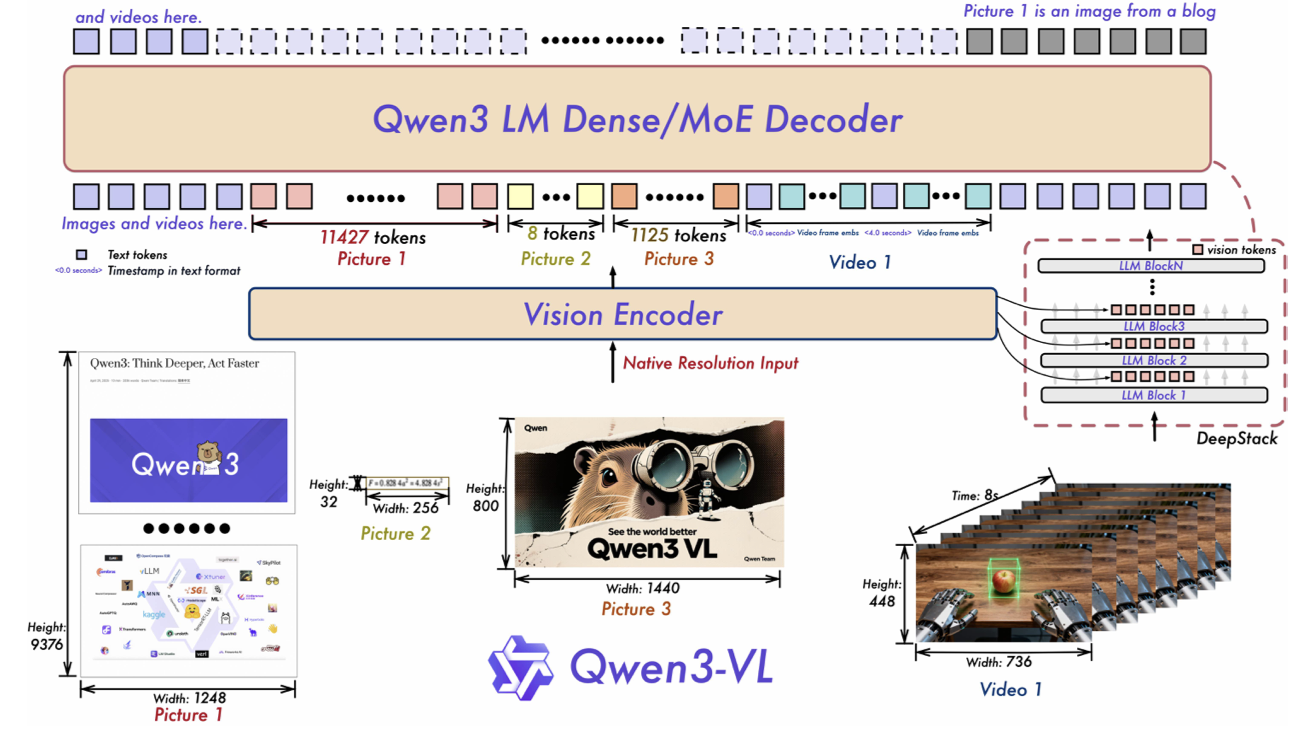
\includegraphics[width=\linewidth]{figures/qwen3vl.png}}%
    {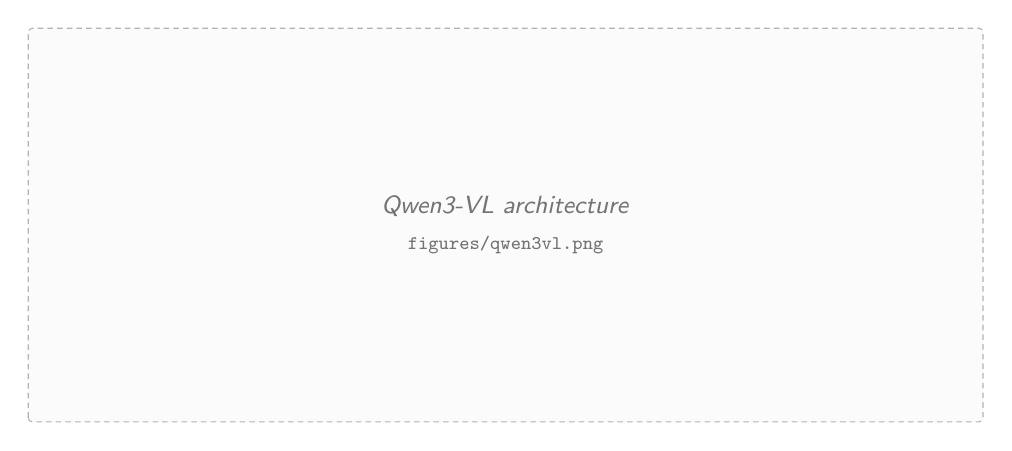
\begin{tikzpicture}[x=\linewidth, y=1cm]
      \draw[draw=black!30, line width=0.4pt, rounded corners=1.5pt,
            fill=gray!3, dash pattern=on 2pt off 1.5pt]
        (0,0) rectangle (1, 5.0);
      \node[font=\small\sffamily, text=black!55, align=center]
        at (0.5, 2.5)
        {\textit{Qwen3-VL architecture}\\[2pt]\scriptsize \texttt{figures/qwen3vl.png}};
    \end{tikzpicture}}%
  \caption[Qwen3-VL architecture]{Qwen3-VL: a distinct vision
  module (preprocessor, vision blocks with interleaved M-RoPE,
  and patch merger) injects multi-level features into the
  language backbone through the DeepStack mechanism. Reproduced
  from the Qwen3-VL technical report \citep{qwen2025qwen3vl}.}
  \label{fig:arch-qwen3vl}
\end{figure}

Disclosure along these axes is structurally asymmetric.
Open-weight families publish technical reports that document
the pipeline end to end, whereas closed frontier families
publish only system cards
\citep{anthropic2026systemcard, openai2025gpt5card,
deepmind2026gemini3card} that leave the encoder, resolution
policy, token budget and connector architecture undisclosed.
Any evaluation that would attribute an observed output to a
specific pipeline stage by reading internal states therefore
has, at the frontier, no internal states to read.

\section{How do today's VLMs reason about what they see, and is it impacted by language?}
\label{sec:bg-reason}

Reasoning in a vision-language model is autoregressive text
generation conditioned on a vision-token prefix. At each
decoding step the backbone's self-attention layers attend over
a sequence that concatenates projected vision tokens with the
text prompt, so every generated token is a function of both
channels jointly. Any cognitive operation the model performs
on a figure is realised, mechanically, as attention-weighted
retrieval from this joint prefix.

\begin{figure}[!ht]
  \centering
  \begin{tikzpicture}[
    font=\footnotesize\sffamily,
    vtok/.style={draw=blue!40, fill=blue!6, line width=0.4pt,
      rounded corners=1pt, minimum width=0.55cm, minimum height=0.45cm,
      inner sep=0pt},
    ttok/.style={draw=orange!50, fill=orange!8, line width=0.4pt,
      rounded corners=1pt, minimum width=0.55cm, minimum height=0.45cm,
      inner sep=0pt},
    gtok/.style={draw=black!35, fill=gray!5, line width=0.4pt,
      rounded corners=1pt, minimum width=0.55cm, minimum height=0.45cm,
      inner sep=0pt},
    arr/.style={-{Latex[length=1.3mm,width=1mm]}, draw=black!35,
      line width=0.3pt},
    lab/.style={font=\scriptsize\sffamily, text=black!55}
  ]
    \foreach \i in {1,...,6} {
      \node[vtok] (v\i) at (\i*0.6, 0) {};
    }
    \foreach \j/\l in {1/$q_1$,2/$q_2$,3/$q_3$,4/$q_4$} {
      \node[ttok] (t\j) at (4.2 + \j*0.6, 0) {\tiny \l};
    }
    \node[gtok, draw=red!45, fill=red!8] (g1) at (7.5, 0) {\tiny $y_1$};
    \node[lab, below=2pt of v3, xshift=0.15cm] {vision tokens (from encoder)};
    \node[lab, below=2pt of t2, xshift=0.15cm] {text prompt};
    \node[lab, below=2pt of g1] {next token};

    \foreach \i in {1,...,6} {
      \draw[arr, blue!40, opacity=0.55] (v\i.north) to[bend left=20] (g1.north);
    }
    \foreach \j in {1,...,4} {
      \draw[arr, orange!50, opacity=0.65] (t\j.north) to[bend left=20] (g1.north);
    }
  \end{tikzpicture}
  \caption[Joint vision-plus-text prefix at decoding time]{At
  each decoding step the next token is produced by
  self-attention over a single sequence formed by concatenating
  the projected vision tokens with the text-prompt tokens;
  cross-modal reasoning is, mechanically, attention-weighted
  retrieval over this joint prefix.}
  \label{fig:joint-prefix}
\end{figure}

Three prompting regimes are layered on this substrate. Under
\emph{direct-answer} prompting the model emits its answer
immediately, and whatever reasoning occurs is implicit in the
transformer computation between the prefix and the first
output token. Under \emph{chain-of-thought} (CoT) prompting
\citep{wei2022chain} the model first emits a natural-language
rationale and then the answer, so that each rationale token
re-attends to the vision tokens and spreads visual retrieval
across more decoding steps. Multimodal extensions couple this
loop to image-space scaffolding. Multimodal-CoT
\citep{zhang2023mmcot} interleaves rationale generation with
visual features in a two-stage procedure; Set-of-Mark prompting
\citep{yang2023som} overlays enumerated marks on the image so
the rationale can reason over discrete regions by reference;
and visual chain-of-thought \citep{shao2024visualcot}
conditions the model to emit region crops during reasoning,
effectively re-querying the encoder on sub-regions.

Language enters this pipeline at three structurally distinct
layers and perturbs reasoning at each. At the \emph{pixel}
layer the vision encoder processes non-Latin scripts through
the same fixed patch grid it was pretrained on predominantly
for English, so fine-grained symbol recognition (Cyrillic
diacritics, Chinese logographs at axis-label size, German
compound axis labels) degrades before any language-specific
reasoning takes place. At the \emph{token} layer the
backbone's tokeniser fragments non-English text into finer
subword units, lengthening the sequence over which a claim
about the figure is represented and diluting the backbone's
lexical priors. At the \emph{prior} layer the pretraining
distribution is itself English-dominant, so for an
underdetermined chart the conditional distribution over
continuations is biased toward English-plausible content. The
three layers are largely independent and a given perturbation
can act on any one or on all three at once.

\section{Behavioural Dynamics of VLMs under Challenging or Adversarial Vision Conditions}
\label{sec:bg-behave}

The pipeline above does not degrade uniformly when an image
is ambiguous, partially obscured, or placed in tension with
its prompt. Figure~\ref{fig:model-responses} captures the
spread in a single probe on the multilingual sunburst of
Figure~\ref{fig:hero}, in which the target label
\emph{Teleplay Characters} has been deliberately blurred.

\begin{figure}[H]
  \centering
  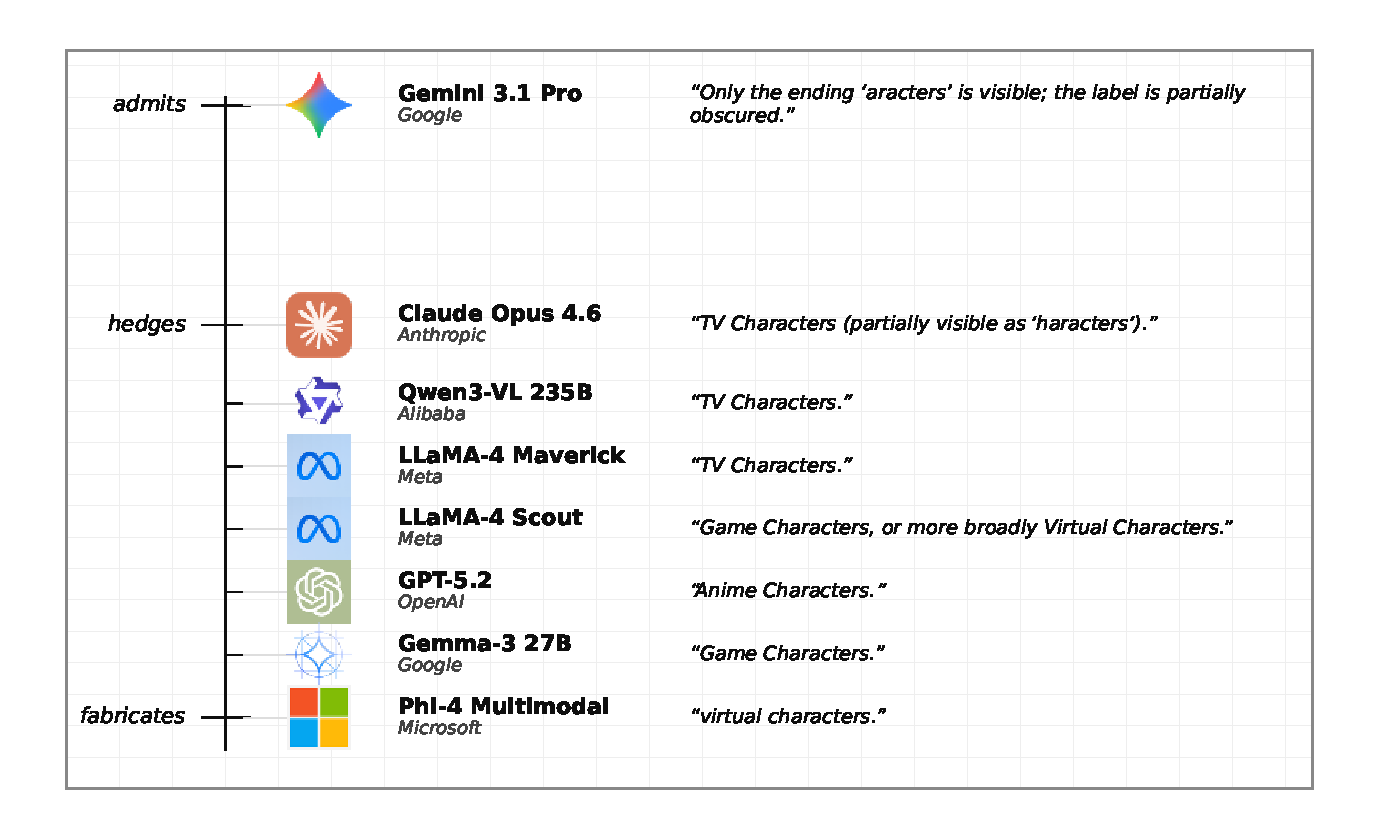
\includegraphics[width=0.95\textwidth]{figures/model_responses_admittance.pdf}
  \caption[Model responses to a single admittance probe.]{%
    Eight contemporary VLMs answering the same probe on the
    sunburst chart from Figure~\ref{fig:hero}. The probe asks
    which outer-ring category sits between Movie Characters
    and Novel Characters; the ground-truth answer
    (\emph{Teleplay Characters}) is deliberately blurred in
    the image. Models are placed on a vertical scale from
    explicit admission at the top through hedged
    acknowledgement to confident fabrication at the bottom,
    with vertical gap proportional to how far each response
    sits from an admission of the obscured label. Each row
    shows the model, its family, and the exact response
    emitted.}
  \label{fig:model-responses}
\end{figure}

Only Gemini 3.1 Pro explicitly flags the obscured label and
reports the visible fragment. Claude Opus 4.6 hedges with a
partial acknowledgement but still commits to a guess. The two
models whose guess is semantically closest to ground truth
(Qwen3-VL 235B and LLaMA-4 Maverick, both answering
\emph{TV Characters}) sit just beneath Claude, followed by
LLaMA-4 Scout's multi-hedge and then confident fabrications
from GPT-5.2 (Anime), Gemma-3 27B (Game) and Phi-4 (a vague
\emph{virtual characters}). Frontier families differ
substantially in how their outputs change under stress, and
the range of observed dispositions is wider than a single
accuracy number suggests.

A model may hold a veridical reading when a leading caption
pulls against it or quietly revise its description to match
the asserted position, the visual analogue of
\emph{sycophancy} \citep{sharma2023sycophancy}. It may combine
image evidence with domain convention to reach a conclusion
the pixels do not literally state, a capacity often unlocked
only under chain-of-thought decoding. And when the pixels
required to answer are blurred, occluded, or absent, it may
acknowledge the gap and qualify its answer, or produce a
confident substitute whose tone is indistinguishable from its
answers on unperturbed inputs. The text-only counterpart of
that last disposition is the calibration behaviour of
\citet{kadavath2022know}; a matching property on an impaired
perceptual prefix is not guaranteed by the architecture.

What the empirical literature does not yet supply is a
structured way of reading these dispositions off a model's
outputs across a controlled stress surface, and that is the
gap addressed by the behavioural framework developed in
Chapter~4.

\section{Evaluating VLM Vision Proficiencies}
\label{sec:bg-evaluate}

Open-ended visual evaluation of a VLM places two demands on
the measurement apparatus: a rubric more expressive than
binary accuracy, since the capabilities indexed in
\S\ref{sec:bg-behave} are not correct-or-incorrect; and a
grading procedure that avoids a human annotator for every
candidate, since modern multilingual and perturbation-based
evaluations routinely yield tens of thousands of outputs.

The reference rubric is Multidimensional Quality Metrics
(MQM), introduced by \citet{lommel2014multidimensional} for
machine translation and since extended across natural-language
generation. Each error is tagged with a category from a fixed
typology (accuracy, fluency, terminology, style) and a
severity weight (minor, major, critical), and a scalar quality
score is computed as a weighted aggregation of the tagged
errors. The apparatus transfers to figure description, with
the typology becoming visual fidelity, completeness and
clarity and the severity weighting distinguishing a misread
tick from a fabricated series.

Human MQM annotation does not scale, and the standard
alternative is the \emph{LLM-as-judge} paradigm
\citep{zheng2023judging}, in which a strong general-purpose
model grades candidates against a rubric. The paradigm is
reproducible and, under careful deployment, reaches
human-level agreement on several tasks, but exhibits
documented systematic biases: self-preference toward a judge's
own family style \citep{wataoka2024selfpref}; position bias
that persists across most judges \citep{zheng2023judging}; and
length and verbosity biases that reward elaboration largely
independent of correctness. Randomising candidate position,
averaging across position swaps, and aggregating across a
heterogeneous judge ensemble form the methodological baseline
for open-ended VLM evaluation.
